\section{Token Bucket Dynamics}
The dynamics of the filter can be described using the matrix $H$ as
%
\begin{flalign}
    P_n=P_{n-1}H
\end{flalign} 
%
where $P_n$ contains the probabilities of being in each of the states of the queue at each time in the queue and $P_{n-1}$ contains the probabilities in the previous time.

As time approaches infinity, $P_n$ converges. This converged vector of probabilities is called $\Pi$ and fulfills the balance equation 
\begin{flalign}
    \Pi=\Pi H \label{eq:pieq}
\end{flalign} 
%
To be able to calculate the mean queue length, mean waiting time and the packet loss probability, it is necessary to find $\Pi$, that gives the converged probabilities of each of the queue.
    
This is done solving \autoref{eq:pieq} and forcing $\sum_{i=0}^{L} \Pi$ to be 1 (L is the queue length).

The first step is to calculate H. It contains the probabilities of moving among the different states in the queue. Since the queue lengths are sampled each token period, $\frac{1}{r_\mathrm{t}}$, the probabilities for a number of packets arriving can be calculated as
%
\begin{flalign}
    A_j=P(a_n=j)=\frac{(\lambda \frac{1}{r_\mathrm{t}})^j}{j!} \exp(-\lambda \frac{1}{r_\mathrm{t}})
\end{flalign}
%
where $a_n$ is the number of arrivals from a Poisson stream in the service
period, $\lambda$ is the arrival rate of packets to the filter.
%
\begin{flalign}
H=
\begin{bmatrix}
A_0 + A_1 & A_2 & A_3 & A_4 & ... & ... & 1-\sum_{0}^{L}A_j  \\
A_0 & A_1 & A_2 & A_3 & ... & ... & 1-\sum_{0}^{L-1}A_j \\
0   & A_0 & A_1 & A_2 & ... & ... & 1-\sum_{0}^{L-2}A_j \\
0   & 0   & A_0 & A_1 & ... & ... & 1-\sum_{0}^{L-3}A_j \\
... & ... & ... & ... & ... & ... & ... \\
0   & 0   & 0   & 0   & ... & A_0 & 1-A_0
\end{bmatrix}
\end{flalign}
%
Once it is calculated it is possible to solve for $\Pi$ in \autoref{eq:pieq}

The mean queue length, mean waiting time and packet loss probability are given by:
%
\begin{flalign}
    \bar{Q}&=\sum_{i=0}^{L} \Pi_i i \\
    \bar{W}&=\frac{\bar{Q}}{\lambda(1-PLP)} \\
    PLP&=\Pi_L
\end{flalign}

\subsection{Rear Camera}
The $H$ matrix in the case of the rear camera is $9\times9$ as the queue can hold a maximum of 8 packets. The mean queue length, mean waiting time and PLP is found following the procedure above.
%
\begin{flalign}
    \bar{Q} &= 0.1635\ \mathrm{packets} \\
    \bar{W} &= 0.0065\ \mathrm{s}\\
    PLP &= 3.1616 \cdot 10^{-5}
\end{flalign}
%
The estimated queue lengths and mean delay have been found using the TrueTime Simulation by averaging their values in a 50 seconds simulation. These are seen below.
%
\begin{flalign}
	\bar{Q}&=0.1490\ \mathrm{packets}  \nonumber\\
	\bar{W}&=0.0026\ \mathrm{s} \nonumber\\
	Q_{\mathrm{max}}&=8\ \mathrm{packets}  \nonumber\\
	W_{\mathrm{max}}&=0.1312\ \mathrm{s} \nonumber
\end{flalign}
%
The figures below show how the queue and the delay evolved in the simulation.
%
\begin{figure}[H]
	\captionbox
	{
		Queue length of the rear camera in the simulation.
		\label{fig:queueRC}
	}
	{
		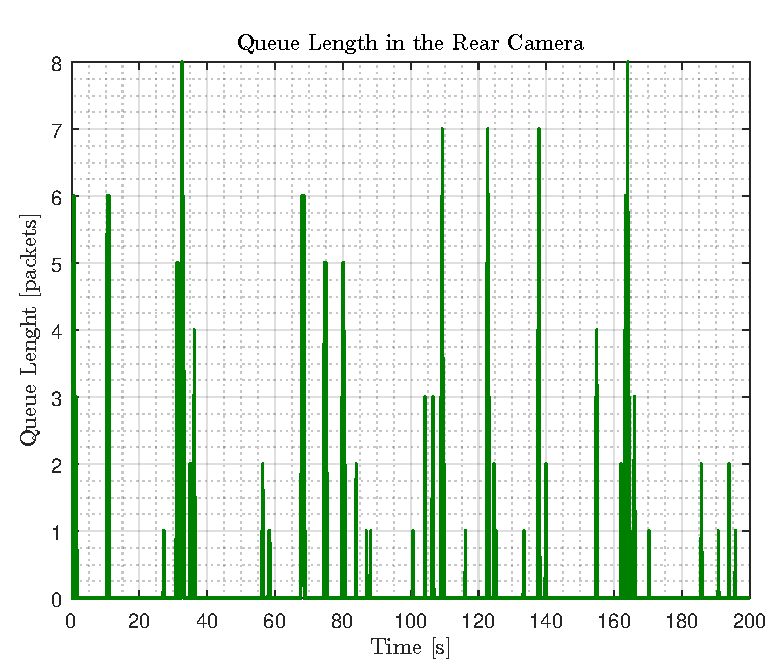
\includegraphics[width=.4\textwidth]{figures/queueRC}
	}
	\hspace{5pt}
	\captionbox
	{
		Waiting time of the rear camera in the simulation.
		\label{fig:timeRC}
	}
	{
		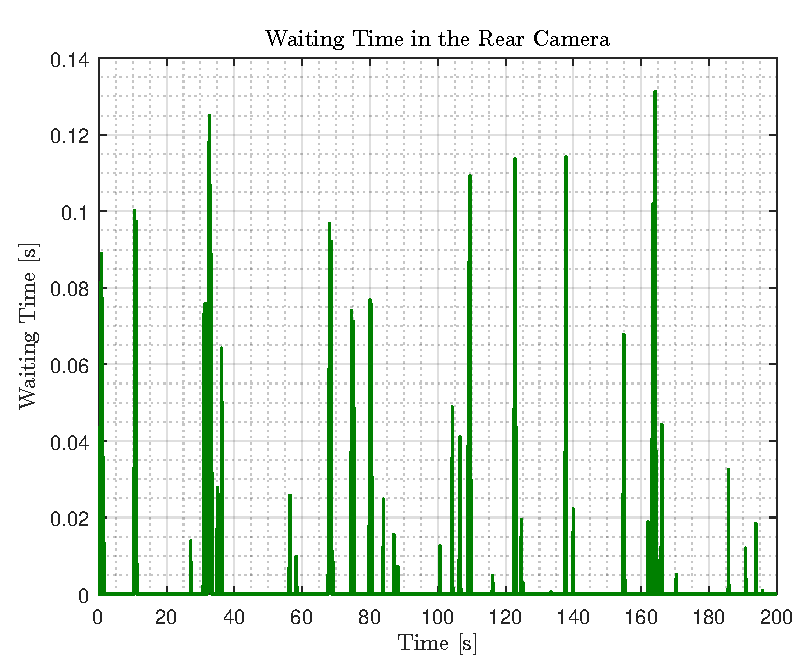
\includegraphics[width=.4\textwidth]{figures/timeRC}
	}
\end{figure}

\subsection{Multimedia System}
In the multimedia case, the $H$ matrix is $6\times6$ as the queue length is 5. The analytical values for the mean queue length, mean waiting time and PLP are found similarly as for the multimedia.
%
\begin{flalign}
    \bar{Q} &= 0.1331 \ \mathrm{packets}\\
    \bar{W} &= 0.0067 \ \mathrm{s}\\
    PLP &= 1.4426 \cdot 10^{-4}
\end{flalign}
%
The estimated queue lengths and mean delay have been found using the TrueTime Simulation following the same procedure as for the rear camera.
%
\begin{flalign}
	\bar{Q}&=0.0763\ \mathrm{packets}  \nonumber\\
	\bar{W}&=0.0019\ \mathrm{s} \nonumber\\
	Q_{\mathrm{max}}&=5\ \mathrm{packets}  \nonumber\\
	W_{\mathrm{max}}&=0.0999\ \mathrm{s} \nonumber
\end{flalign}
%
The figures below show how the queue and the delay evolved in the simulation.
%
\begin{figure}[H]
	\captionbox
	{
		Queue length of the rear camera in the simulation.
		\label{fig:queueMultimedia}
	}
	{
		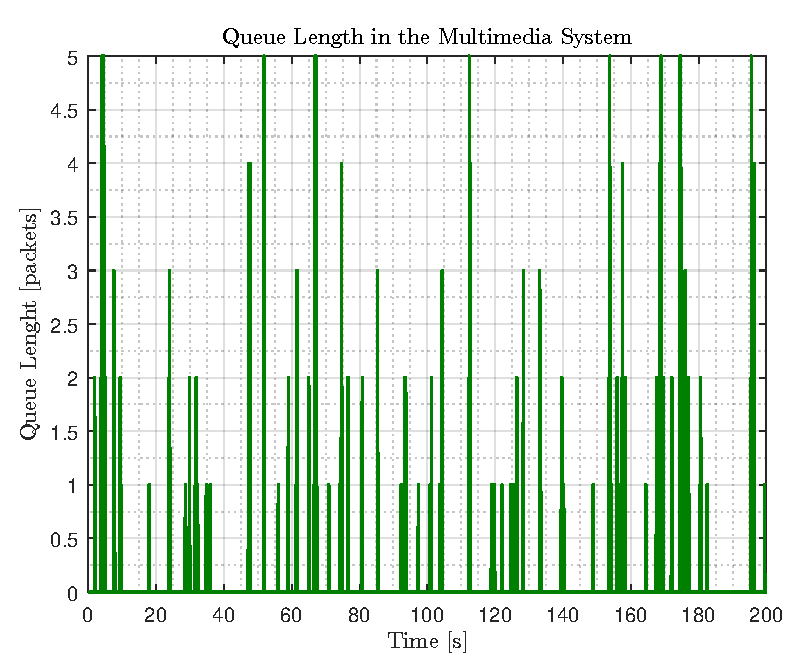
\includegraphics[width=.4\textwidth]{figures/queueMultimedia}
	}
	\hspace{5pt}
	\captionbox
	{
		Waiting time of the rear camera in the simulation.
		\label{fig:timeMultimedia}
	}
	{
		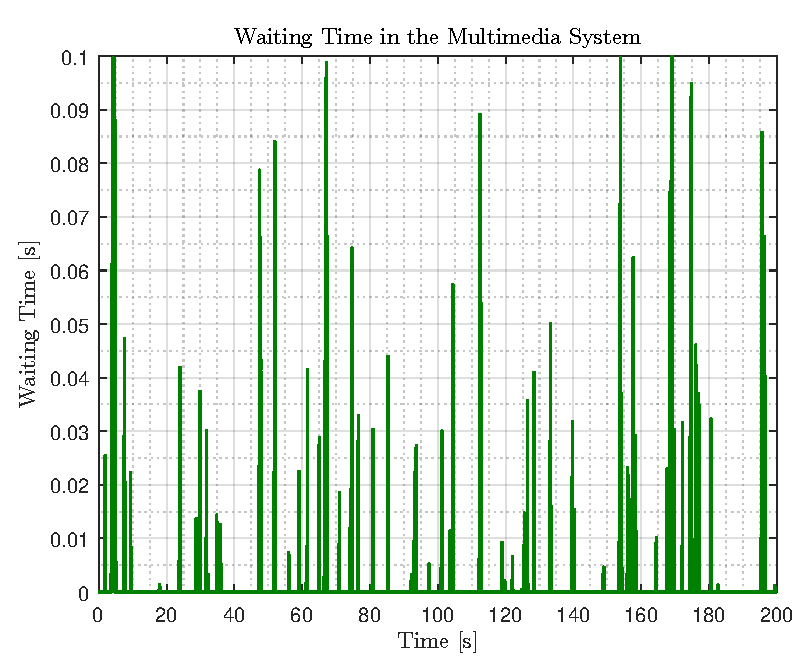
\includegraphics[width=.4\textwidth]{figures/timeMultimedia}
	}
\end{figure}